\documentclass[tikz,border=8pt]{standalone}
\usetikzlibrary{arrows.meta,calc}
\definecolor{bg}{HTML}{FCFCFA}
\definecolor{beam}{HTML}{D7263D}
\definecolor{beamret}{HTML}{F28C28}
\definecolor{mirror}{HTML}{4A5A6A}
\definecolor{mirrorface}{HTML}{BFD7EA}
\definecolor{glass}{HTML}{CFE6F3}
\definecolor{laser}{HTML}{2F3640}
\definecolor{screen}{HTML}{F6F1E7}
\definecolor{ink}{HTML}{233044}
\begin{document}
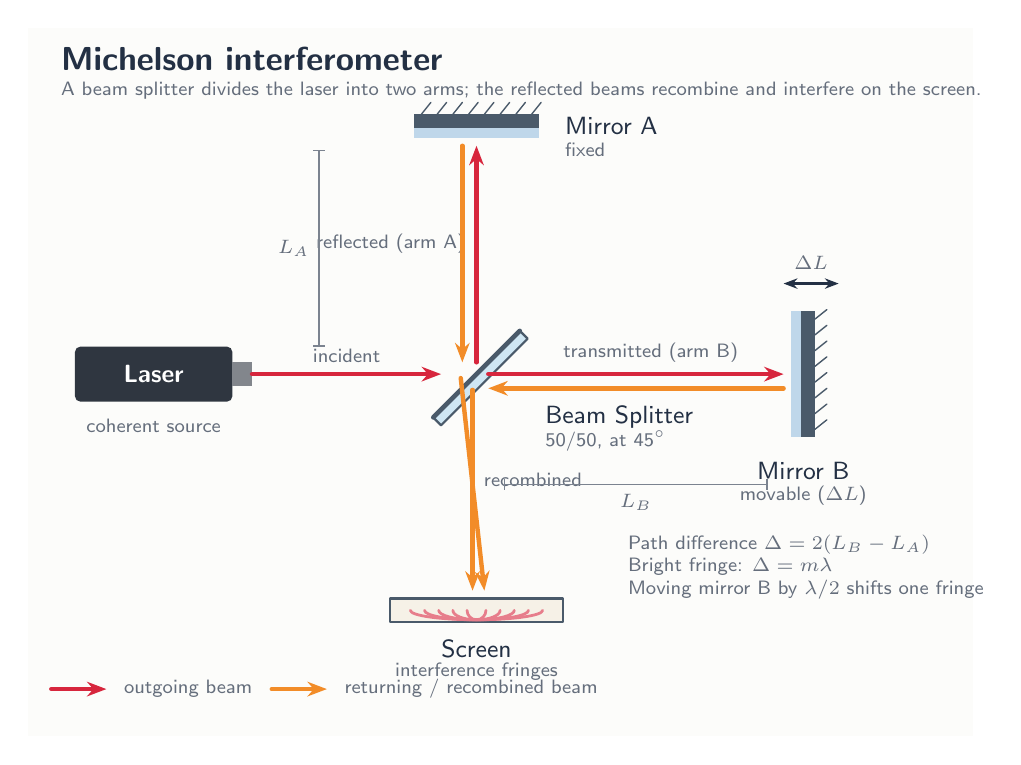
\begin{tikzpicture}[x=1cm,y=1cm,line cap=round,line join=round,
  ray/.style={-{Stealth[length=7pt]},line width=1.6pt,beam},
  rayret/.style={-{Stealth[length=7pt]},line width=1.6pt,beamret},
  lbl/.style={font=\sffamily\small,text=ink},
  sub/.style={font=\sffamily\scriptsize,text=ink!70!white},
  dim/.style={{Bar[width=4pt]}-{Bar[width=4pt]},line width=0.5pt,ink!60!white}]
  \fill[bg] (-1.2,-1.6) rectangle (10.8,7.4);
  \node[font=\sffamily\bfseries\large,text=ink,anchor=west] at (-0.9,7.0) {Michelson interferometer};
  \node[sub,anchor=west] at (-0.9,6.6) {A beam splitter divides the laser into two arms; the reflected beams recombine and interfere on the screen.};

  \coordinate (BS) at (4.5,3.0);
  \coordinate (MA) at (4.5,6.0);   % mirror A (top arm)
  \coordinate (MB) at (8.5,3.0);   % mirror B (right arm)
  \coordinate (SC) at (4.5,0.0);   % screen (bottom)

  % ---- laser (left) ----
  \fill[laser,rounded corners=2pt] (-0.6,2.65) rectangle (1.4,3.35);
  \fill[laser!60!white] (1.4,2.85) rectangle (1.65,3.15);
  \node[lbl,text=white,font=\sffamily\bfseries\small] at (0.4,3.0) {Laser};
  \node[sub] at (0.4,2.35) {coherent source};

  % ---- beam splitter (45 deg glass plate) ----
  \fill[glass,draw=mirror,line width=0.8pt] ($(BS)+(-0.55,-0.55)$) -- ($(BS)+(0.55,0.55)$) -- ($(BS)+(0.65,0.45)$) -- ($(BS)+(-0.45,-0.65)$) -- cycle;
  \draw[mirror,line width=1.6pt] ($(BS)+(-0.55,-0.55)$) -- ($(BS)+(0.55,0.55)$);
  \node[lbl,anchor=west] at ($(BS)+(0.75,-0.55)$) {Beam Splitter};
  \node[sub,anchor=west] at ($(BS)+(0.75,-0.85)$) {50/50, at 45$^\circ$};

  % ---- mirror A (top, horizontal face) ----
  \fill[mirrorface] ($(MA)+(-0.8,0)$) rectangle ($(MA)+(0.8,0.12)$);
  \fill[mirror] ($(MA)+(-0.8,0.12)$) rectangle ($(MA)+(0.8,0.3)$);
  \foreach \i in {-0.7,-0.5,...,0.7}{\draw[mirror,line width=0.5pt] ($(MA)+(\i,0.3)$) -- ($(MA)+(\i+0.12,0.45)$);}
  \node[lbl,anchor=west] at ($(MA)+(1.0,0.15)$) {Mirror A};
  \node[sub,anchor=west] at ($(MA)+(1.0,-0.15)$) {fixed};

  % ---- mirror B (right, vertical face, movable) ----
  \fill[mirrorface] ($(MB)+(0,-0.8)$) rectangle ($(MB)+(0.12,0.8)$);
  \fill[mirror] ($(MB)+(0.12,-0.8)$) rectangle ($(MB)+(0.3,0.8)$);
  \foreach \i in {-0.7,-0.5,...,0.7}{\draw[mirror,line width=0.5pt] ($(MB)+(0.3,\i)$) -- ($(MB)+(0.45,\i+0.12)$);}
  \node[lbl,anchor=north] at ($(MB)+(0.15,-1.0)$) {Mirror B};
  \node[sub,anchor=north] at ($(MB)+(0.15,-1.3)$) {movable ($\Delta L$)};
  \draw[{Stealth[length=5pt]}-{Stealth[length=5pt]},line width=0.8pt,ink] ($(MB)+(-0.1,1.15)$) -- ($(MB)+(0.6,1.15)$);
  \node[sub,anchor=south] at ($(MB)+(0.25,1.2)$) {$\Delta L$};

  % ---- screen / detector (bottom) ----
  \fill[screen,draw=mirror,line width=0.8pt] ($(SC)+(-1.1,-0.15)$) rectangle ($(SC)+(1.1,0.15)$);
  \node[lbl,anchor=north] at ($(SC)+(0,-0.25)$) {Screen};
  \node[sub,anchor=north] at ($(SC)+(0,-0.55)$) {interference fringes};
  % fringe rings drawn on the screen surface
  \foreach \r in {0.12,0.3,0.48,0.66,0.84}{\draw[beam!60!white,line width=1pt] ($(SC)+(-\r,0)$) arc [start angle=180,end angle=360,x radius=\r,y radius=0.12];}

  % ---- rays: outgoing (red) ----
  \draw[ray] (1.65,3.0) -- ($(BS)+(-0.45,0)$) node[sub,midway,above] {incident};
  % transmitted straight to mirror B
  \draw[ray] ($(BS)+(0.15,0)$) -- ($(MB)+(-0.1,0)$) node[sub,pos=0.55,above] {transmitted (arm B)};
  % reflected up to mirror A
  \draw[ray] ($(BS)+(0,0.15)$) -- ($(MA)+(0,-0.1)$) node[sub,pos=0.55,left] {reflected (arm A)};

  % ---- rays: returning (orange, slightly offset for readability) ----
  \draw[rayret] ($(MB)+(-0.1,-0.18)$) -- ($(BS)+(0.15,-0.18)$);
  \draw[rayret] ($(MA)+(-0.18,-0.1)$) -- ($(BS)+(-0.18,0.15)$);
  % recombined beam to the screen
  \draw[rayret] ($(BS)+(-0.05,-0.2)$) -- ($(SC)+(-0.05,0.25)$) node[sub,pos=0.45,right] {recombined};
  \draw[rayret] ($(BS)+(-0.2,-0.05)$) -- ($(SC)+(0.1,0.25)$);

  % ---- arm length dimensions ----
  \draw[dim] (2.5,3.35) -- (2.5,5.85) node[sub,midway,left] {$L_A$};
  \draw[dim] (4.85,1.6) -- (8.2,1.6) node[sub,midway,below] {$L_B$};

  % ---- notes ----
  \node[sub,anchor=west,align=left] at (6.3,0.55) {Path difference $\Delta = 2(L_B - L_A)$\\Bright fringe: $\Delta = m\lambda$\\Moving mirror B by $\lambda/2$ shifts one fringe};
  \draw[ray] (-0.9,-1.0) -- (-0.2,-1.0); \node[sub,anchor=west] at (-0.1,-1.0) {outgoing beam};
  \draw[rayret] (1.9,-1.0) -- (2.6,-1.0); \node[sub,anchor=west] at (2.7,-1.0) {returning / recombined beam};
\end{tikzpicture}
\end{document}
